\chapter{Monte Carlo Simulation of Physics Processes at ATLAS}
\label{chap:MCSimulation}

\indent Simulated Monte Carlo (MC) samples are used to model the signal and background processes in this analysis.  In general, a MC generator program calculates the hard interaction matrix element up to a certain degree of accuracy (leading order (LO), next-to-leading order (NLO), next-to-next leading order (NNLO), etc.)  Another program simulates the formation of parton showers through the fragmentation and hadronization of colored partons at low energy scales.  The matrix element calculation at high energy scales and the parton shower calculations at low energy scales are then matched to one another using a prescribed matching scheme.  \\

\indent A parton density function (PDF) is used to describe the internal structures of the colliding protons. An underlying event tune is used to describe the different parameters associated with the parton shower including the amount of ISR/FSR emitted and the amount of multiple parton interactions. Different scales such as the factorization and renormalization scales must also be set as input parameters.  \\

\indent  Because the LHC is operating at such high instantaneous luminosities, there are around 25 proton-proton interactions per bunch crossing.  Most of these pile-up interactions have low amounts of momentum transfer between the protons and are modeled by overlaying additional minimum-bias interactions on top of the hard scattering interaction.  Further details on the modeling of pile-up interactions can be found in the section \ref{sec:MC:PileUp}. \\

\indent After MC generation, the ATLAS detector is simulated using the \geant 4 program.\cite{Geant}  The simulated detector response is then reconstructed into physics objects using ATLAS reconstruction algorithms described in chapter \ref{chap:reconstruction}.  Further details on detector simulation can be found in the section \ref{sec:MC:DET}.

\indent A summary of MC generation programs and parameters are given in Table \ref{tab:mc_samples1}.  Details on the MC generation process for each signal and background MC are covered in sections \ref{sec:MC:Sig} - \ref{sec:MC:diboson}.  \\  %A full list of the samples that are used is given in Appendix~\ref{App:DatasetList}.

\begin{table}[h!]
  \caption{Overview of the nominal simulated samples. Generator refers to the MC generator program used for the matrix element calculation. fragm./hadron. refers to the program that simulates the formation of parton showers through the fragmentation and hadronization of colored partons.  PDF set is the parton distribution function used to model the internal structure of the proton. UE Tune describes the different parameters used in the modeling of the parton shower. The cross section order refers to the degree of accuracy the matrix element calculation is performed to.}
  \label{tab:mc_samples1}
  \centering
  \small
  \begin{tabular}{cccc} \hline
    Process & \multicolumn{2}{c}{Generator} & fragm./hadron. \\% & PDF set  & UE Tune & Cross section order\\
    \hline 
    \hline
    Stop Signal & \multicolumn{2}{c}{{\sc MadGraph5\_aMC\/@NLO}} & {\sc Pythia} 8 \\ %& NNPDF2.3 & A14 & LO  & \\ 
    $t\bar{t}$ & \multicolumn{2}{c}{{\sc Powheg-Box} v2} & {\sc Pythia} 6 \\%& CT10  & {\sc Perugia 2012} & NLO & \\ 
    Single-Top & \multicolumn{2}{c}{{\sc Powheg-Box} v2} & {\sc Pythia} 6 \\%& CT10  & {\sc Perugia 2012} & NLO & \\ 
    $W/Z$+jets & \multicolumn{2}{c}{{\sc Sherpa} 2.2.1} & {\sc Sherpa}  \\%& NNPDF3.0NNLO & Default & NLO & \\ 
    Diboson & \multicolumn{2}{c}{{\sc Sherpa} 2.2} & {\sc Sherpa} \\%& CT10 & Default & LO\\ 
    $t\bar{t}+V$ & \multicolumn{2}{c}{{\sc MadGraph5\_aMC\/@NLO}} & {\sc Pythia} 8 \\%& NNPDF3.0NNLO & A14 & NLO \\ 
    \hline \hline
       & & &  \\ \hline
    Process & PDF set  & UE Tune & Cross section order \\ \hline \hline
    stop signal & NNPDF2.3 & A14 & LO   \\ 
    $t\bar{t}$ & CT10  & {\sc Perugia 2012} & NLO  \\ 
    single-top & CT10  & {\sc Perugia 2012} & NLO \\ 
    $W/Z$+jets & NNPDF3.0 NNLO & Default & NLO  \\ 
    diboson & CT10 & Default & LO \\ 
    $t\bar{t}+V$  & NNPDF3.0 NNLO & A14 & NLO \\ 
    \hline
  \end{tabular}
  \end{table}

\section{Detector Simulation}
\label{sec:MC:DET}

\indent Two types of detector simulations are used.  \geant 4 \cite{Geant} is used to perform the detector simulation for all background samples.  For signal MC, a fast simulation framework is used in the interest of reducing computing time.\cite{ATLFAST}  In the fast simulation framework, the majority of the detector is still simulated with \geant 4 with the exception of jets in the electromagnetic and hadronic calorimeters.  Instead of simulating individual particle showers in the calorimeters, a predetermined parameterized description of the showers are used.  The fast simulation framework was validated against full \geant 4 simulation for several selected signal samples and found to agree in observed kinematics.  \\

\indent  ATLAS performance groups which measure the detector and reconstruction performance may recommend reweighting different MC samples depending on better or worse then expected detector performance.  The following variables are reweighted to account for known differences between data and simulation: the lepton trigger efficiency, lepton reconstruction efficiency, lepton momentum scale, lepton isolation, and the b-tagging efficiency. \\

\section{Pile-Up Simulation}
\label{sec:MC:PileUp}

\indent Because the LHC is operating at such high instantaneous luminosities, there are around 25 proton-proton interactions per bunch crossing.  Most of these interactions have low amounts of momentum transfer between the protons but still deposit energy in the detector.  In order to understand the properties of these additional interactions, ATLAS records inelastic p-p interactions, called minimum-bias interactions, with no particular bias to any one kind of event.  \\

\indent All ATLAS simulation is produced with a varying number of minimum-bias interactions overlaid on top of the hard scattering interaction.  The minimum bias interactions are supposed to mimic the pile-up interactions.  The distribution of additional overlaid minimum bias interactions is reweighted so that the distribution of pile-up interactions matches in data and MC.  \\

\section{Signal Monte Carlo Generation}
\label{sec:MC:Sig}

\indent We use {\sc MadGraph5\_aMC\/@NLO} to calculate the matrix element of the stop signal MC to leading order accuracy (LO).\cite{Madgraph}  Up to two additional QCD partons are included in the matrix element calculation, making the total hard scattering process $pp \rightarrow {\stop}\bar{\stop} + j + j $.   \\

\indent Stop decays are treated differently depending on the mass splitting between the stop and its decay products.  The different stop decays considered in this analysis are shown in the Feynman diagrams in Figure \ref{fig:feynDiagModels}. \\

\begin{figure}[h!]
  \begin{center}
  \begin{subfigure}[b]{0.35\textwidth}  
    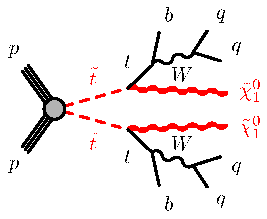
\includegraphics[width=\textwidth]{figures/feynDiag/stst-bqqbqqN1N1-tt.eps}
               \caption{ }
    \end{subfigure}
      \begin{subfigure}[b]{0.35\textwidth}      
    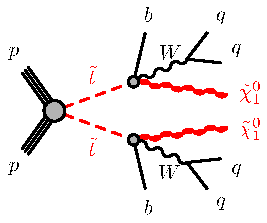
\includegraphics[width=\textwidth]{figures/feynDiag/stst-bqqbqqN1N1-3body.eps}
               \caption{ }
    \end{subfigure}
       \begin{subfigure}[b]{0.35\textwidth}  
      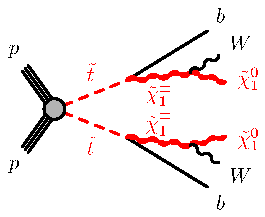
\includegraphics[width=\textwidth]{figures/feynDiag/stst-bbWWN1N1.eps}
               \caption{ }
    \end{subfigure}
\end{center}
\caption{The decay topologies of the signal models considered in this analysis.  The decay mode depends on the mass splitting between stop ($\stop$) and neutralino ($\ninoone$).   If the mass splitting is larger then $m_t$, then a real top maybe produced in (a) the 2 body decay $\stop\rightarrow t\ninoone$. If the mass splitting is too small then a stop may decay through (b) a virtual top to ${\stop}\rightarrow bW\ninoone$.  The stop decaying into b-quark plus chargino ($\chinoonepm$) channel shown in (c) is also considered in mixed decay interpretations. }
\label{fig:feynDiagModels} 
\end{figure}

\indent If $m_{\stop} - m_{\ninoone} \ge m_{t}$, then the top can be produced on shell. \pythiaeight\cite{Pythia8} performs the 2 body ${\stop} \rightarrow t \ninoone$ decay and subsequent decays of the top.  $m_{t}$ is set to $172.5 \gev$.  This process has the advantage of being computationally much faster than including the stop decays as part of the matrix element calculation.  \\ %However it has the disadvantage of assuming that the stop width is zero.  The zero stop width assumption differs from the true stop width case by less then $5$\% in the distributions of all relevant kinematic variables.  The nominal stop width in the simplified model is $1/10$ the width of the top and so the stop width represent only a small smearing on the distribution of $m_{t}$ and $\MET$ compared of the one produced by the top width. \\

\indent If $m_{\stop} - m_{\ninoone} < m_{t}$, then the top must be produced off shell.   \pythiaeight\ cannot perform the 3 body $\stop \rightarrow b W \ninoone$ decay or the 4 body $\stop \rightarrow b f f \ninoone$ decay where the $f$ stands for any fermion that can result from a $W$ decay.  Instead we use \madspin\cite{Madspin} to perform the $\stop \rightarrow b W \ninoone$ or $\stop \rightarrow b ff \ninoone$ decay.  \madspin\ can perform 3 body and 4 body decays with off shell virtual particles as long as the decay are ultimately a series of 2 body decays.  Decaying the stop using \madspin\ also is also much faster then calculating the decay within the matrix element.  \\ %\madspin\ cannot calculate the spin correlations between the two stops but this is not a problem because the stops are scalar particles so no spin correlations exist between the two. \\

\indent After the matrix element calculation and stop decays, the parton shower and hadronization of jets are simulated using \pythiaeight\ with the {\sc EvtGen} v1.2.0 program as an afterburner.  The matching between the matrix element and parton shower jets is preformed with the CKKW-L prescription.   The matching scale is set to $1/4$ the mass of the stop. \\

\indent The internal structure of the proton is modeled with the NNPDF3.0NNLO parton distribution function (PDF) set \cite{NNPDF3.0} with A14 set as the underlying event (UE) tuning parameters\cite{Pythia8tunes}.  The A14 tune optimizes over 10 parameters that vary the amount of ISR, FSR and multiple parton interactions.  The variations are reduced to a 5 variable subset that is found to cover the uncertainty on experimental observables.  Variable 1 mainly covers variation in the modeling of the underlying events.  Variable 2 mainly covers variation in jet structure, and variables 3a, 3b and 3c cover different variations of ISR and FSR production.  All 5 variations are used to quantify the theoretical uncertainties associated with parton shower and multiple parton interactions and are added in quadrature.\\

\indent Signal cross sections are calculated to next-to-leading order in the strong coupling constant with the resummation of soft gluon emission added to next-to-leading-logarithmic accuracy (NLO+NLL).\cite{stopXsec}  An envelope of cross section predictions is produced using different PDF sets and factorization and renormalization scales.  The nominal cross section and the uncertainty are then taken from the median and $1\sigma$ fluctuations around the median within the envelope.  \\

\indent Signal samples are generated to cover the entire stop and neutralino mass phase space that we may be sensitive to.  Stop samples are generated at every 50 $\gev$ $m_{\stop}$ intervals for stop masses between 200 and 700 GeV.  At each stop mass value, five samples with different ${\Delta}m = m_{\stop} - m_{\ninoone}$ are simulated to cover a wide corridor of phase space around ${\Delta}m$ equals the top quark mass ($m_{t}$) line: ${\Delta}m = m_{t} - 82.5 \gev, m_{t} - 52.5 \gev, m_{t} - 22.5 \gev, m_{t} - 7.5 \gev, m_{t}+0.5 \gev,  m_{t}+15.5 \gev, m_{t}+27.5 \gev$.  An extra row of $m_{\stop} = 225 \gev$ samples is also produced to better estimate the 95\% confidence limit at low stop masses. \\

\section{SM Background Monte Carlo Generation}
\label{sec:MC:Bkg}

\subsection{Standard Model $\ttbar$ Monte Carlo Generation}

\indent The nominal $\ttbar$ samples are generated using \textsc{Powheg-Box} v.2.\cite{PowhegTTbar}  The matrix element calculation is computed to NLO accuracy and includes the $pp \rightarrow \ttbar + j$ process where the $j$ represents an one additional emitted parton.  The top quark mass is set to $172.5 \gev$ and the proton substructure is modeled by the CT10 NLO PDF set \cite{CT10} for the hard scattering process.  The hard scattering renormalization and factorization scales are set to the generator default of $\sqrt{(m_{t})^2 + (p_{T t})^2}$.  \\

\indent \pythia~6 version 6.427 simulates the parton shower, hadronization and underlying event.\cite{Pythia6}  We use the Perugia 2012 tune \cite{Perugia2012} and the corresponding leading order CTEQ6L1 PDF set \cite{CTEQ6L1} in \pythia~6.  The resummation damping factor or $h_{damp}$, used by \textsc{Powheg} to control the matrix element and parton shower matching and the amount of high-$\pt$ ISR/FSR, is set to $m_{t}$. \\

\indent $\ttbar$ cross sections are calculated to NNLO accuracy in the strong coupling constant with the resummation of soft gluon emissions added to NNLL accuracy using the \textsc{Top++v2.0} program.\cite{topXsec}  Similar to the signal MC generation, an envelope of cross sections is produced for different PDF sets including MSTW2008NNLO, CT10 NNLO and NNPDF2.3 NNLO.  Variations in the renormalization and factorization scales, strong coupling constant, and top quark mass are also included in the envelope.  The median of envelope is taken as the nominal $\ttbar$ cross section and the $1\sigma$ variation in the envelope is taken as the $\ttbar$ cross section uncertainty.  \\

\indent In addition to the total cross section uncertainty, a number of $\ttbar$ samples are produced to study the variation in the shapes of $\ttbar$ kinematic distributions. \\
\indent  Two additional samples called radHi and radLo are produced to study the variation in the total amount of ISR/FSR.  These samples have different renormalization and factorization scales than the nominal sample (x0.5 to radHi and x2 to radLo) in order to simulate $\ttbar$ with more/less ISR/FSR emissions. The radHi sample also increases the $h_{damp}$ parameter, which controls the matching between the matrix element and parton shower calculations, from the nominal $m_{t}$ to $2 \times m_{t}$. \\

\indent We study the variation of the parton shower simulation using a \textsc{Powheg+Herwigg++} $\ttbar$ sample. The hard scattering matrix element calculation is the same as the nominal \textsc{Powheg+\pythia~6} sample.  However the parton shower, fragmentation and hadronization is now performed with \textsc{Herwigg++} program with the UE-EE-5 parameter tune.\cite{Herwigg,CTEQ6L1}  \\%\textsc{Herwigg++} provides an alternative method to perform the parton shower calculation when compared to nominal {\sc Pythia} 6 program. \\  %The PDF used for the matrix element calculation is still CT10 NLO and the calculation is still performed with \textsc{Powheg-Box}v.2 with the $h_{damp} = m_{t}$.  \\

\indent Variations in the hard scattering matrix element calculation are studied by comparing the nominal to a sample generated using the \sherpa~\cite{sherpa} program.  \sherpa~gives an alternative method to calculating both the matrix element and parton shower when compared to the nominal \textsc{Powheg+\pythia~6} sample.  The same CT10 NLO PDF set is used for \sherpa~and the nominal sample.  However \sherpa~uses the default UE tune derived by the \sherpa~team instead of the nominal Perugia 2012 UE tune. \\ 

\indent Non-overlapping samples that are filtered in to $\met$ are generated to increase statistics at high $\met$ where our analysis resides.  These samples are then merged after simulation to form a  continuous $\met$ distribution. \\

\subsection{Standard Model Single-Top Monte Carlo Generation}

\indent Like the nominal $\ttbar$ sample, the nominal single-top samples are also simulated using \textsc{Powheg-Box} v.2\cite{PowhegST_st,PowhegST_wt} with the \pythia~6 program being used for hadronization and parton showering.  Similar to the $\ttbar$ sample, the single-top samples use the CT10 NLO PDF set and the Perugia 2012 set of UE tune parameters. \\

\indent Unlike the $\ttbar$ samples, single-top samples are produced separately according to production channels.  Three production channels exist, including the s-channel, t-channel and the Wt channel.  The largest contribution to our analysis comes from the Wt channel.  \\

\indent The NLO calculation of the $pp \rightarrow Wt$ process includes contributions from $ pp \rightarrow \ttbar \rightarrow t + b + W$ process.  However $ pp \rightarrow \ttbar \rightarrow t + b + W$ is already included in our simulation of $\ttbar$ and including it here would be double counting.  We can subtract out the $\ttbar$ contribution at either the amplitude level (DR scheme) or at the matrix element level (DS scheme).  Subtracting at the matrix element level also remove any potential interference between the single-top $pp \rightarrow Wt$ process and the $ pp \rightarrow \ttbar \rightarrow t + b + W$ process.  Subtracting at the amplitude level does not remove those interferences.  Both schemes violate formal gauge invariance and there isn't a consensus on the correct procedure.  The nominal single-top sample is generated with the DR scheme and another sample is generated with the DS scheme.  We compare the difference between the two samples to quantify the uncertainty due to the single-top and $\ttbar$ interference. \\

\indent RadHi and radLo samples are also produced for single-top to study the variation in single-top ISR and FSR emissions.  These samples are also produced with \textsc{Powheg+\pythia6} but have different renormalization and factorization scales (x0.5 to radHi and x2 to radLo) to simulate more/less ISR/FSR emissions. The radHi sample also increase the $h_{damp}$ parameter from the nominal $m_{t}$ to $2 \times m_{t}$. \\

\indent We study the variation of the parton shower simulation using \textsc{Powheg+Herwigg++} single-top samples.  The hard scattering matrix element calculation has not changed from the nominal.  The PDF used for the matrix element calculation is still CT10 NLO and the calculation is still performed with \textsc{Powheg-Box}v.2 with the $h_{damp} = m_{t}$.  However the parton shower, fragmentation and hadronization is now performed with \textsc{Herwigg++} with the UE-EE-5 underlying event tune.\cite{CTEQ6L1} \\

\subsection{Standard Model $\Wjets$ and $\Zjets$ Monte Carlo Generation}

\indent $\Wjets$ and $\Zjets$ are generated with the \sherpa v2.2.1 program.\cite{sherpa}  The matrix element are calculated for the vector boson plus 0, 1, and/or 2 additional partons at NLO accuracy and 3 and/or 4 additional partons at LO accuracy.  \\

\indent The matrix element calculation is merged with the \sherpa\ parton shower according to the \sc{MEPS@NLO} prescription.  The proton substructure is modeled with the NNPDF3.0 NNLO PDF set and the parton shower tuning defined by \sherpa.\cite{NNPDF3.0}   \\

\indent  We also generate additional samples that include 7 variations on the renormalization and factorization scales.  These variations are used to quantify the theoretical uncertainty on our modeling of the $\Wjets$ and $\Zjets$. \\

\indent  The $\Wjets$ and $\Zjets$ samples are generated in multiple non-overlapping slices of vector boson $\pt$.  The samples are further subdivided depending on the presence of b-jets and c-jets.  These samples are merged after simulation to form a continuous distribution covering all phase space.  This allows us to generate higher statistics in the region of phase space most relevant to our analysis, the region with high-$\pt$ vector bosons and where b and/or c-jets are present. \\

\subsection{Standard Model $\ttbar+V$ Monte Carlo Generation}

\indent $\ttbar+V$, where $V$ is a $W$ or $Z$ boson, MC simulation are generated using the {\sc MadGraph5\_aMC\/@NLO} program with the NNPDF3.0 NLO PDF set.\cite{NNPDF3.0}  The matrix element calculation is performed to NLO accuracy. The parton shower, fragmentation, and hadronization are simulated using \pythiaeight\ with the A14 underlying event tune.  Variations in the hard scattering matrix element calculation are studied by generating another sample using \sherpa\ and comparing its results to the nominal sample.  Variation in renormalization and factorization scales are also produced. \\

\subsection{Standard Model $\ttbar+\gamma$ Monte Carlo Generation}

\indent $\ttbar+\gamma$ samples are generated using the {\sc MadGraph5\_aMC\/@NLO} program with the NNPDF3.0 NLO PDF set.\cite{NNPDF3.0} The matrix element calculation is performed to NLO accuracy. The parton shower, fragmentation, and hadronization are simulated using \pythiaeight\ with the A14 underlying event tune.  The sample is filtered to only generate events at least one high $\pt$ photon.  This sample is then merged with the nominal $\ttbar$ sample to form the $\ttbar+\gamma$ sample.  The events with high $\pt$ photons in the nominal $\ttbar$ samples are removed to avoid double counting. \\

\subsection{Standard Model Diboson Monte Carlo Generation}
\label{sec:MC:diboson}

\indent Dibosons samples are generated using the \sherpa~v2.2 program with CT10 PDF set. \\



